\chapter{Theory}
\label{chp:theory}

\begin{center}
    \textit{This chapter delves into the theoretical foundations of the technologies and methodologies employed in the project. It covers key concepts such as computer vision, image recognition, and the integration of chess analysis tools like \Gls{stockfish}.}    
\end{center}

\section{Literature Review}
\label{sec:literature-review}

As technology continues to evolve, a variety of digital tools and platforms have emerged to enhance the experience of playing and analyzing chess. Leading online platforms such as \textit{chess.com} and \textit{lichess.org} provide global matchmaking, tutorials, and advanced game analysis features, significantly transforming how chess is played and studied. \\

In addition to software-based innovations, physical chessboards have also been modernized through the integration of digital technologies. For example, the use of \gls{rfid} tags enables the digitization of over-the-board games, allowing for automated tracking and broadcasting of moves. \cite{quora:shah} \\

Clono is a tablet-based electronic scoresheet system designed to replace traditional paper scoresheets. It transmits game data to the Clono Server, enabling live online broadcasts of tournaments. Clono offers a secure, affordable, and easy-to-use solution that does not require electronic chessboards, cables, or on-site technical personnel. \cite{clono} \\

Moreover, recent advancements in \gls{ai} have led to the development of applications capable of automating tasks such as piece recognition and game digitization. A notable example is \textit{ChessCam}, a web- and mobile-based application that facilitates rapid, real-time digitization of chess games. Users can either upload pre-recorded video footage or stream live games via a mobile phone or webcam. The application processes the visual input, detects moves, and generates \gls{pgn} files suitable for analysis or archival. \cite{chess:chesscam, lichess:chesscam}

\section{Technologies}
\label{sec:technologies}

\subsection{Version Control}
\label{subsec:version-control}

The use of \gls{git} as a version control system enables collaborative development by allowing multiple developers to work on the same codebase simultaneously. \gls{git} facilitates the maintenance of the code and provides a comprehensive history of all modifications made to the project. These changes are tracked within project containers known as \glspl{repository}, ensuring transparency and accountability throughout the development process. \cite{alphaefficiency:git}

\subsubsection*{Branches}

\subsection{Machine Learning}
\label{sec:machine-learning}

\subsubsection*{Computer Vision}
\label{subsubsec:computer-vision}

As a subfield of \gls{ai}, computer vision focuses on enabling machines to interpret, analyze, and extract meaningful information from visual data, such as digital images and videos. The primary goal of computer vision is to replicate the human ability to perceive, and understand visual information, automating tasks that traditionally require human intelligence (see Figure \ref{fig:computer-vision}). \cite{google:vision, microsoft:vision}

\begin{figure}[h!]
    \centering
    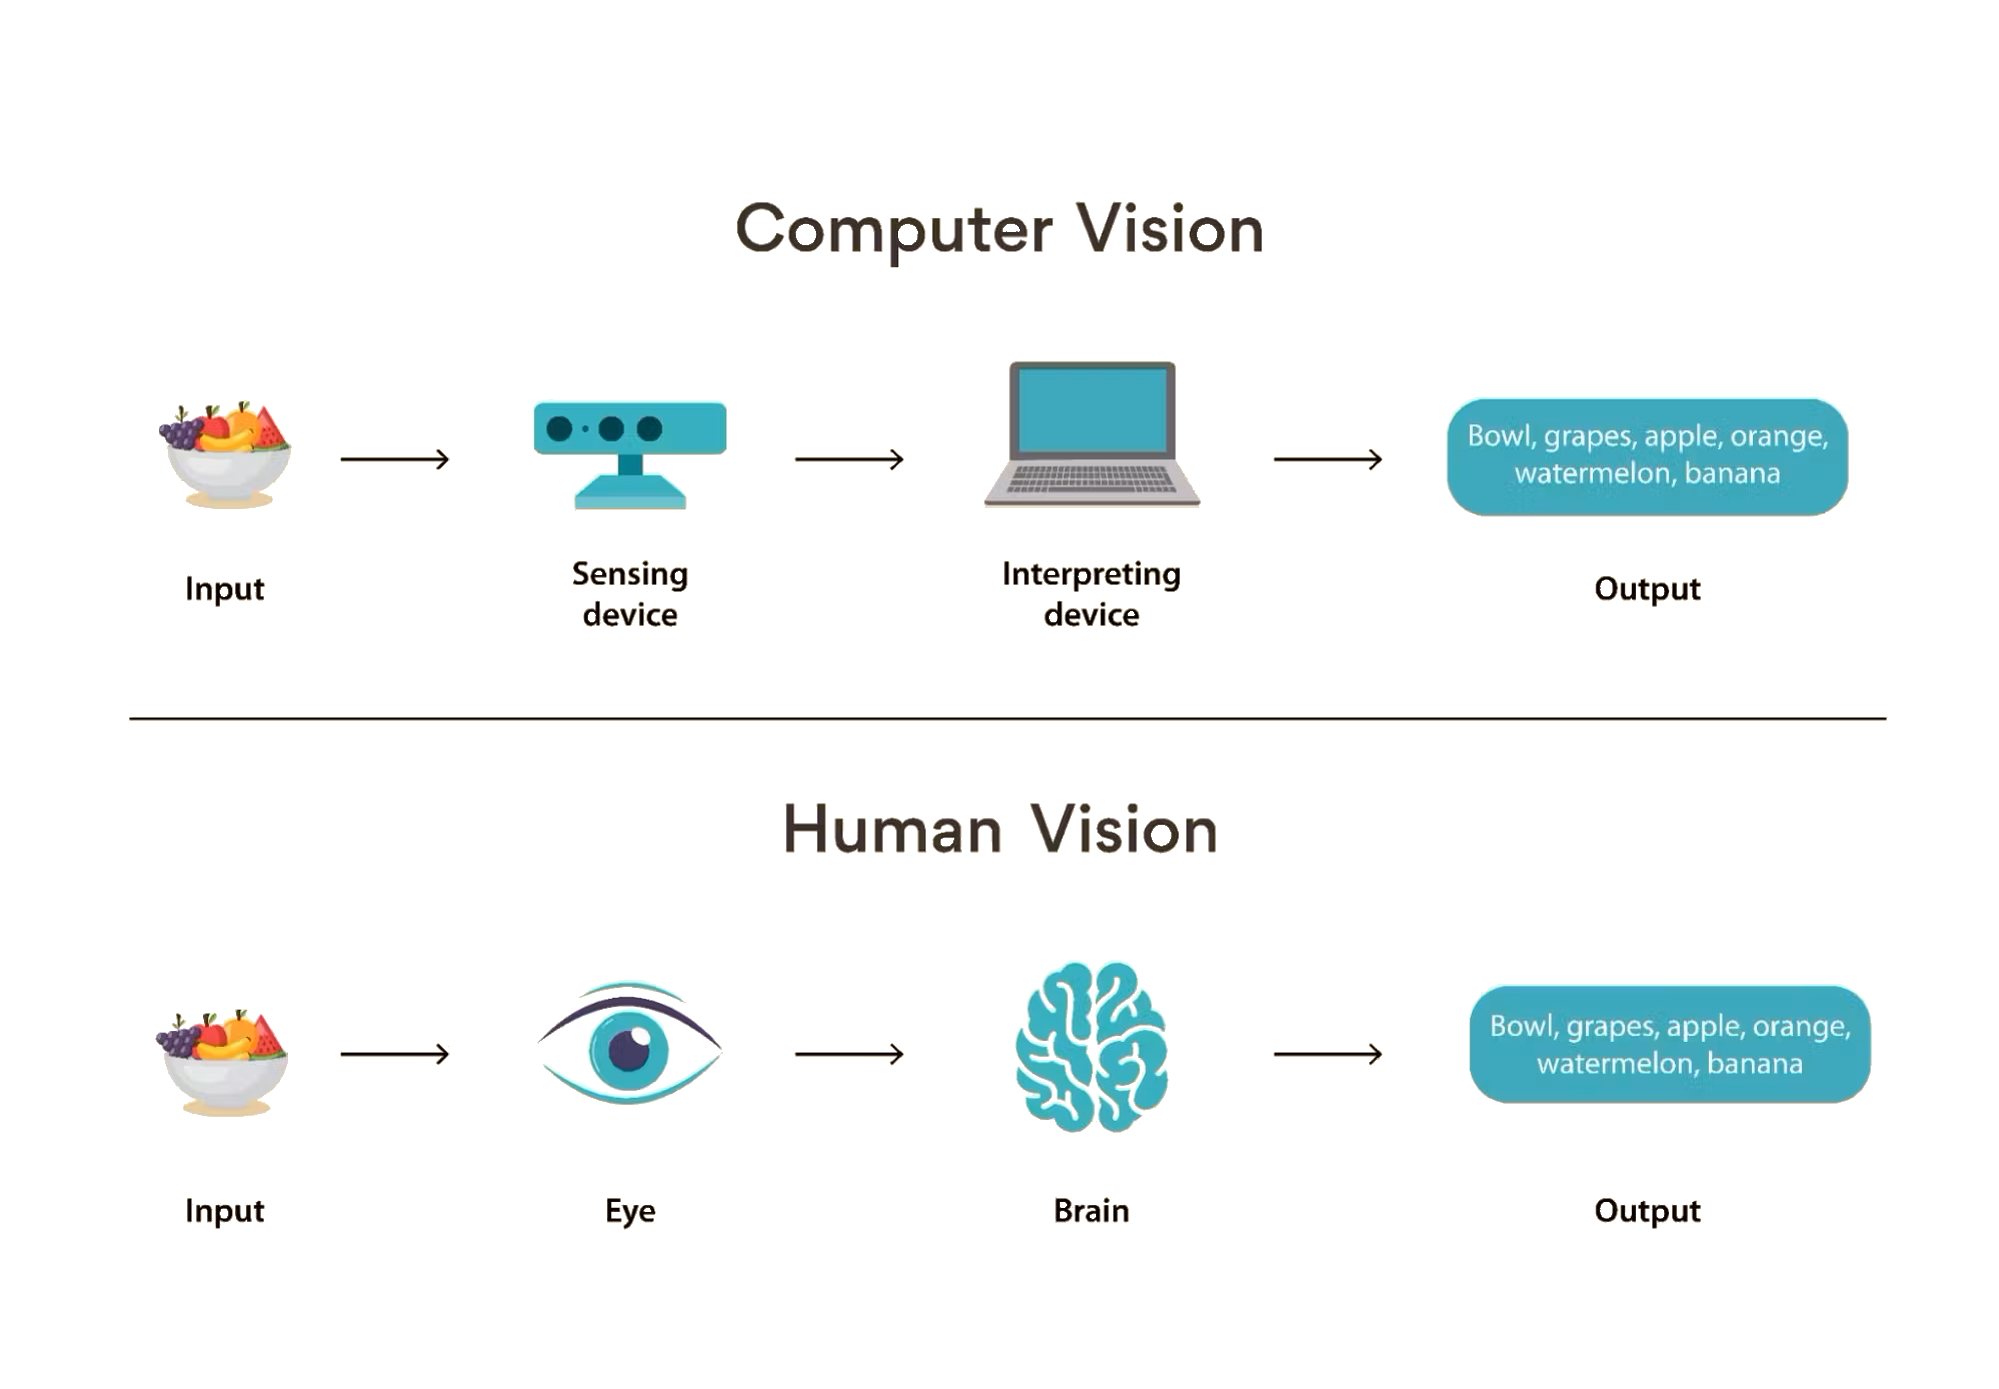
\includegraphics[width=0.75\linewidth]{figures/theory/computer-vision.png}
    \caption[Computer Vision \& Human Vision]{Computer Vision \& Human Vision \cite{turing:computer-vision}}
    \label{fig:computer-vision}
\end{figure}

\subsubsection*{Artificial Neural Network}
\label{subsubsec:artificial-neural-network}

Artificial Neural Networks (ANNs) are a cornerstone of modern \gls{ml}, excelling in processing diverse datasets, including images, audio, and text. Different types of neural networks are tailored for specific tasks. For instance, Recurrent Neural Networks (RNNs), particularly Long Short-Term Memory (LSTM) networks, are effective for sequential data like text or time series. In contrast, \glspl{cnn} are specifically designed for image-related tasks, such as image classification, object detection, and segmentation. Their unique architecture, which includes convolutional layers, enables them to automatically and efficiently extract spatial features from visual data. An example of a \gls{cnn} architecture used to classify handwritten digits is shown in Figure \ref{fig:convolutional-neural-network}. \cite{geeksforgeeks:cnn} \\

\begin{figure}[h!]
    \centering
    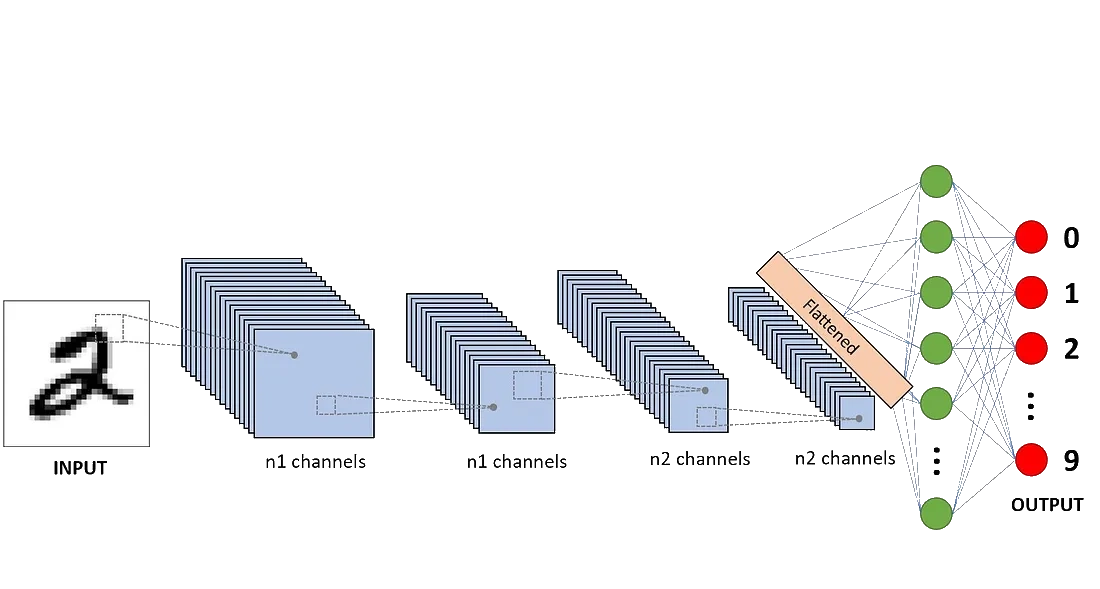
\includegraphics[width=0.75\linewidth]{figures/theory/convolutional-neural-network.png}
    \caption[A CNN sequence to classify handwritten digits]{A CNN sequence to classify handwritten digits \cite{medium:cnn}}
    \label{fig:convolutional-neural-network}
\end{figure}

The versatility and effectiveness of \glspl{cnn} make them a fundamental tool in computer vision applications, ranging from medical imaging to autonomous vehicles. By leveraging their ability to learn hierarchical representations of visual data, \glspl{cnn} have become a driving force behind many advancements in \gls{ai} and \gls{ml}.

\subsubsection*{Supervised Learning}
\label{subsubsec:supervised-learning}

Supervised learning is a fundamental approach for \gls{ml} and \gls{ai}. It involves training a model using labeled data, where each input comes with a corresponding correct output. The process resembles a teacher providing guidance to a student, which is why it is referred to as "supervised" learning. \cite{geeksforgeeks:supervised-learning} \\

The data used in supervised learning is labeled — meaning that it contains examples of both inputs (called features) and correct outputs (labels). The algorithms analyze a large dataset of these training pairs to infer what a desired output value would be when asked to make a prediction on new data. \cite{google:supervised-learning} \\

For instance, consider a scenario where a model is trained to recognize geometric shapes. A labeled dataset would include various shape images paired with their respective names. Through exposure to these examples, the model learns to associate specific visual features with particular shapes. When presented with a new shape, the model attempts to classify it based on its learned knowledge. An overview of this process is illustrated in Figure~\ref{fig:supervised-learning}. If the model makes an incorrect prediction, it can be retrained with additional data to refine its accuracy. \cite{google:supervised-learning} \\

\begin{figure}[h!]
    \centering
    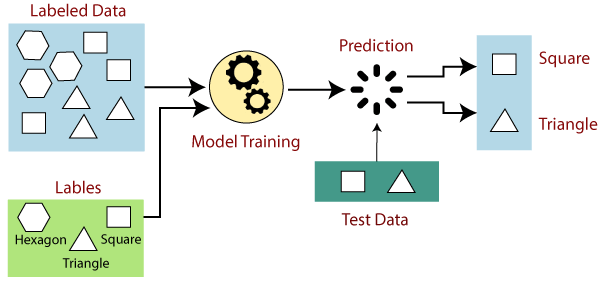
\includegraphics[width=0.75\linewidth]{figures/theory/supervised-learning.png}
    \caption[Supervised Learning process using labeled data]{Supervised Learning process using labeled data \cite{tpointtech:supervised-learning}}
    \label{fig:supervised-learning}
\end{figure}

\newpage

Once the model has been trained and tested, it can be used to make predictions on unknown data based on the previous knowledge it has learned. \cite{google:supervised-learning}

\subsubsection*{Classification}
\label{subsubsec:classification}

Classification is a type of supervised learning used to predict a categorical output variable based on input data. These output variables—known as classes—represent distinct categories, such as "spam" or "not spam", or "disease present" versus "no disease". Classification algorithms are specifically designed to assign new inputs to one of these predefined classes. \cite{google:supervised-learning} \\

A common real-world application of classification is email spam detection. In this case, a supervised learning model is trained using a dataset containing labeled examples of both spam and legitimate emails. The model learns to identify patterns based on various features, such as the sender's address, subject line, and email content. These features, along with their corresponding labels, enable the algorithm to predict whether a new incoming email should be categorized as spam or not. An illustration of this classification process is shown in Figure \ref{fig:classification}. \cite{google:supervised-learning}

\begin{figure}[h!]
    \centering
    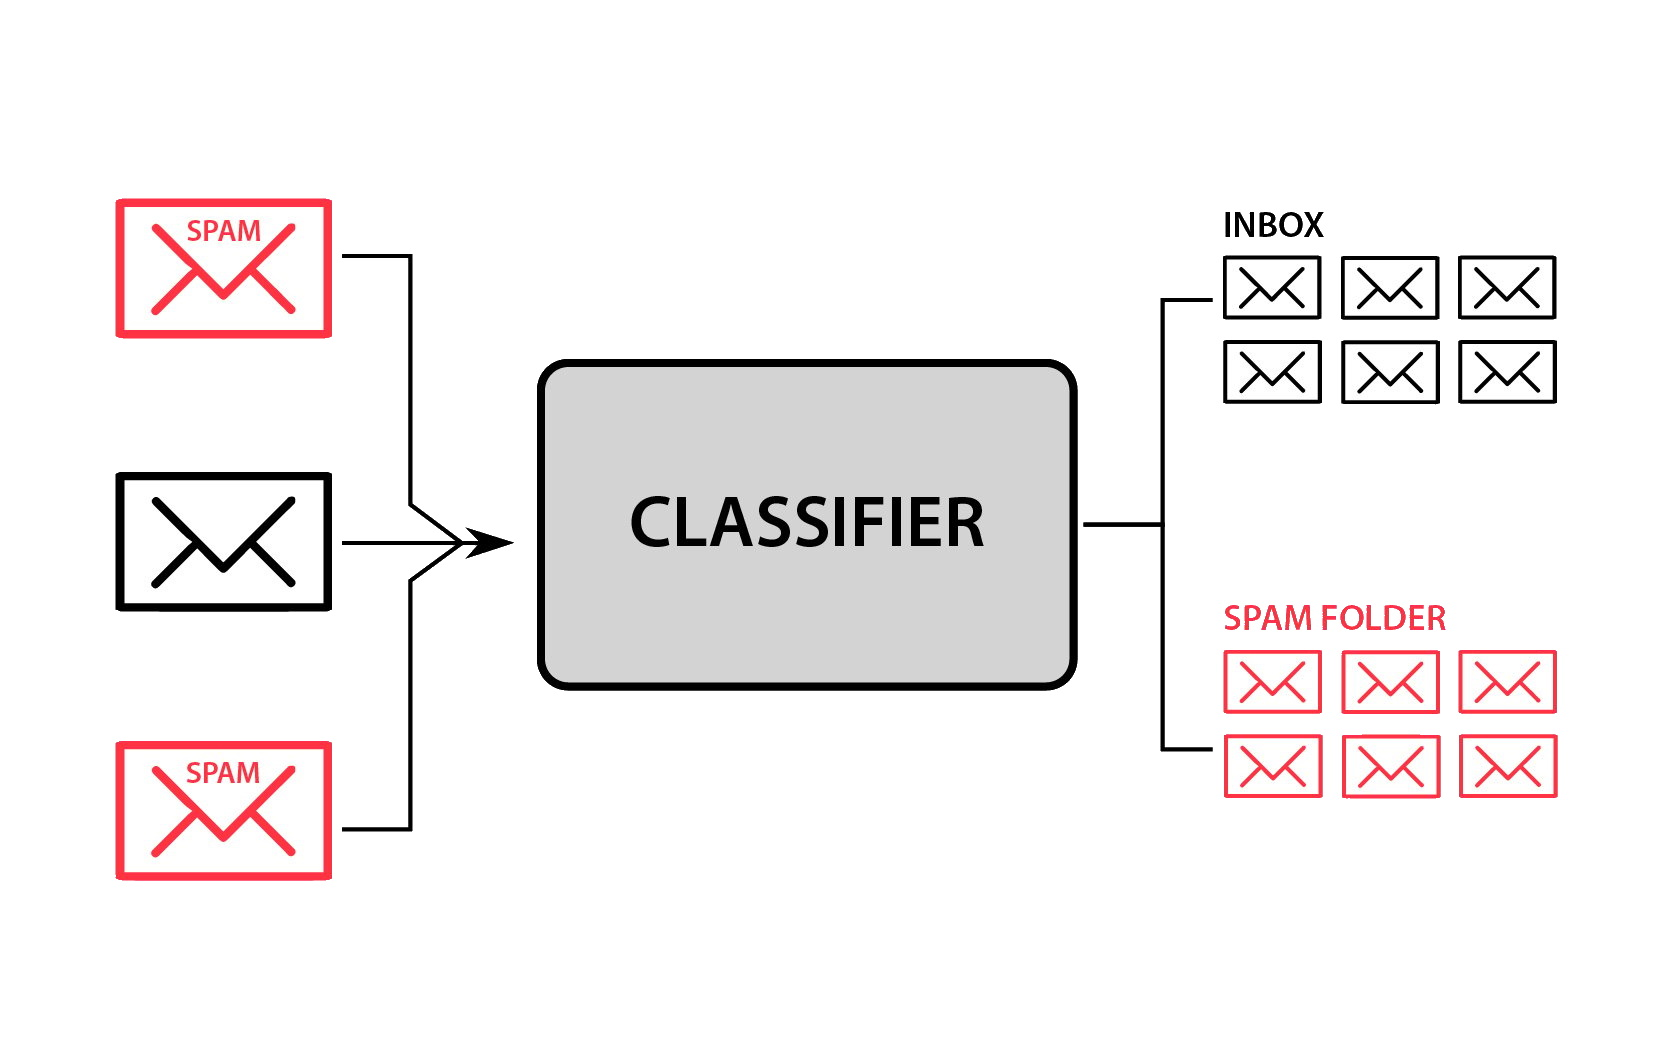
\includegraphics[width=0.75\linewidth]{figures/theory/classification.jpg}
    \caption[Email Classification]{Email Classification \cite{analytixlabs:classification}}
    \label{fig:classification}
\end{figure}

\subsection{Object Detection}

\subsubsection*{Inference} 
Inference refers to the process of using a trained machine learning model to make predictions on new, unseen data. In the context of object detection models, inference involves feeding an input image into the model, which then processes the image and outputs predictions. The predictions typically consist of object classes, confidence scores, and bounding box coordinates. [SOURCE NEEDED] 

\subsubsection*{LeYOLO} 
\gls{leyolo} is a \gls{cnn} designed for real-time object detection. It is a lightweight version of \gls{yolo} where its simplified architecture. allows it to achieve significantly faster inference times. This makes it particularly suitable for real-time applications, where quick detection is more important than achieving the highest possible accuracy. Like its predecessor, it divides an image into a grid, and each cell predicts whether an object is present, along with its bounding box coordinates.  [SOURCE NEEDED]\\

\subsubsection*{Bounding box} 
A bounding box is a rectangular region used to indicate the location of an object within an image. It is typically represented by four values: the center coordinates \((x_c, y_c)\), which define the center of the box, and  the width \((w)\) and height \((h)\), which define the dimensions of the box. In object detection tasks, models predict these coordinates to both localize and classify objects within an image. [SOURCE NEEDED]

\begin{figure}[h!]
    \centering
    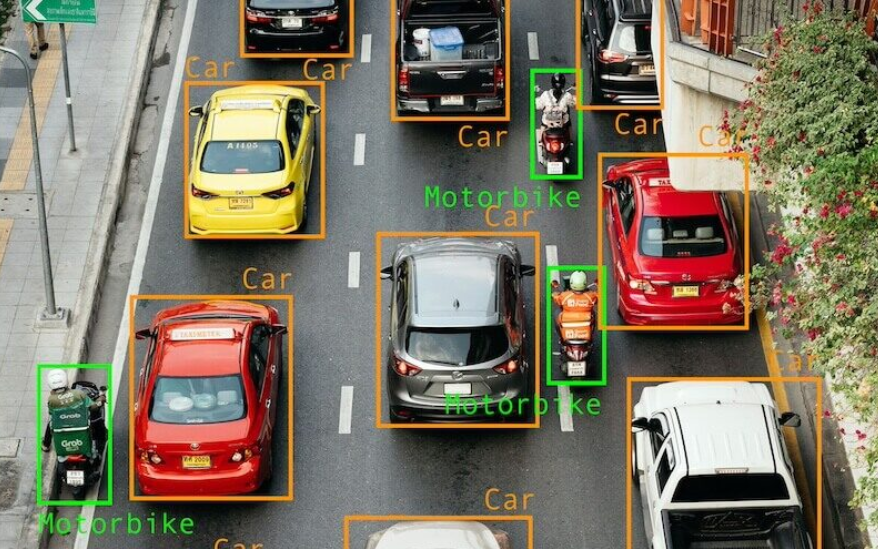
\includegraphics[width=0.8\linewidth]{figures/theory/image-recognition/bbox-example.png}
    \caption[Bounding box example]{Bounding box example \cite{peopleforai:boundingbox}}
    \label{fig:boundingbox}
\end{figure}

\subsubsection*{Anchor Boxes}
Anchor boxes are predefined bounding boxes of various sizes and aspect ratios used as reference points for object detection models. These boxes are placed over the image or feature map to help the model predict the location and dimensions of objects.

Rather than directly predicting bounding boxes, the model predicts offsets (shifts) relative to these anchor boxes, allowing it to adjust the box's position and size to fit the object. The model also predicts a confidence score indicating the likelihood that an object is present.

\begin{figure}[h!]
    \centering
    
\includegraphics[width=0.8\linewidth]{figures/theory/image-recognition/anchor-boxes.png}
    \caption[Anchor boxes example]{Anchor boxes example \cite{thinkautonomous:anchorboxes}}
    \label{fig:anchor-box}
\end{figure}


\subsubsection*{Non-maximum suppression}
\gls{nms} is a post-processing technique used in object detection to eliminate redundant or overlapping bounding boxes . When a model predicts multiple boxes for the same object, \gls{nms} ensures that only the most confident prediction is kept. \\

The algorithm works by first selecting the box with the highest confidence score. It then removes all other boxes that have a high overlap with the selected box. This process is repeated iteratively until no boxes with significant overlap remain. By applying \gls{nms}, object detectors produce cleaner and more accurate results, preventing multiple detections of the same object.


\begin{figure}[h!]
    \centering
    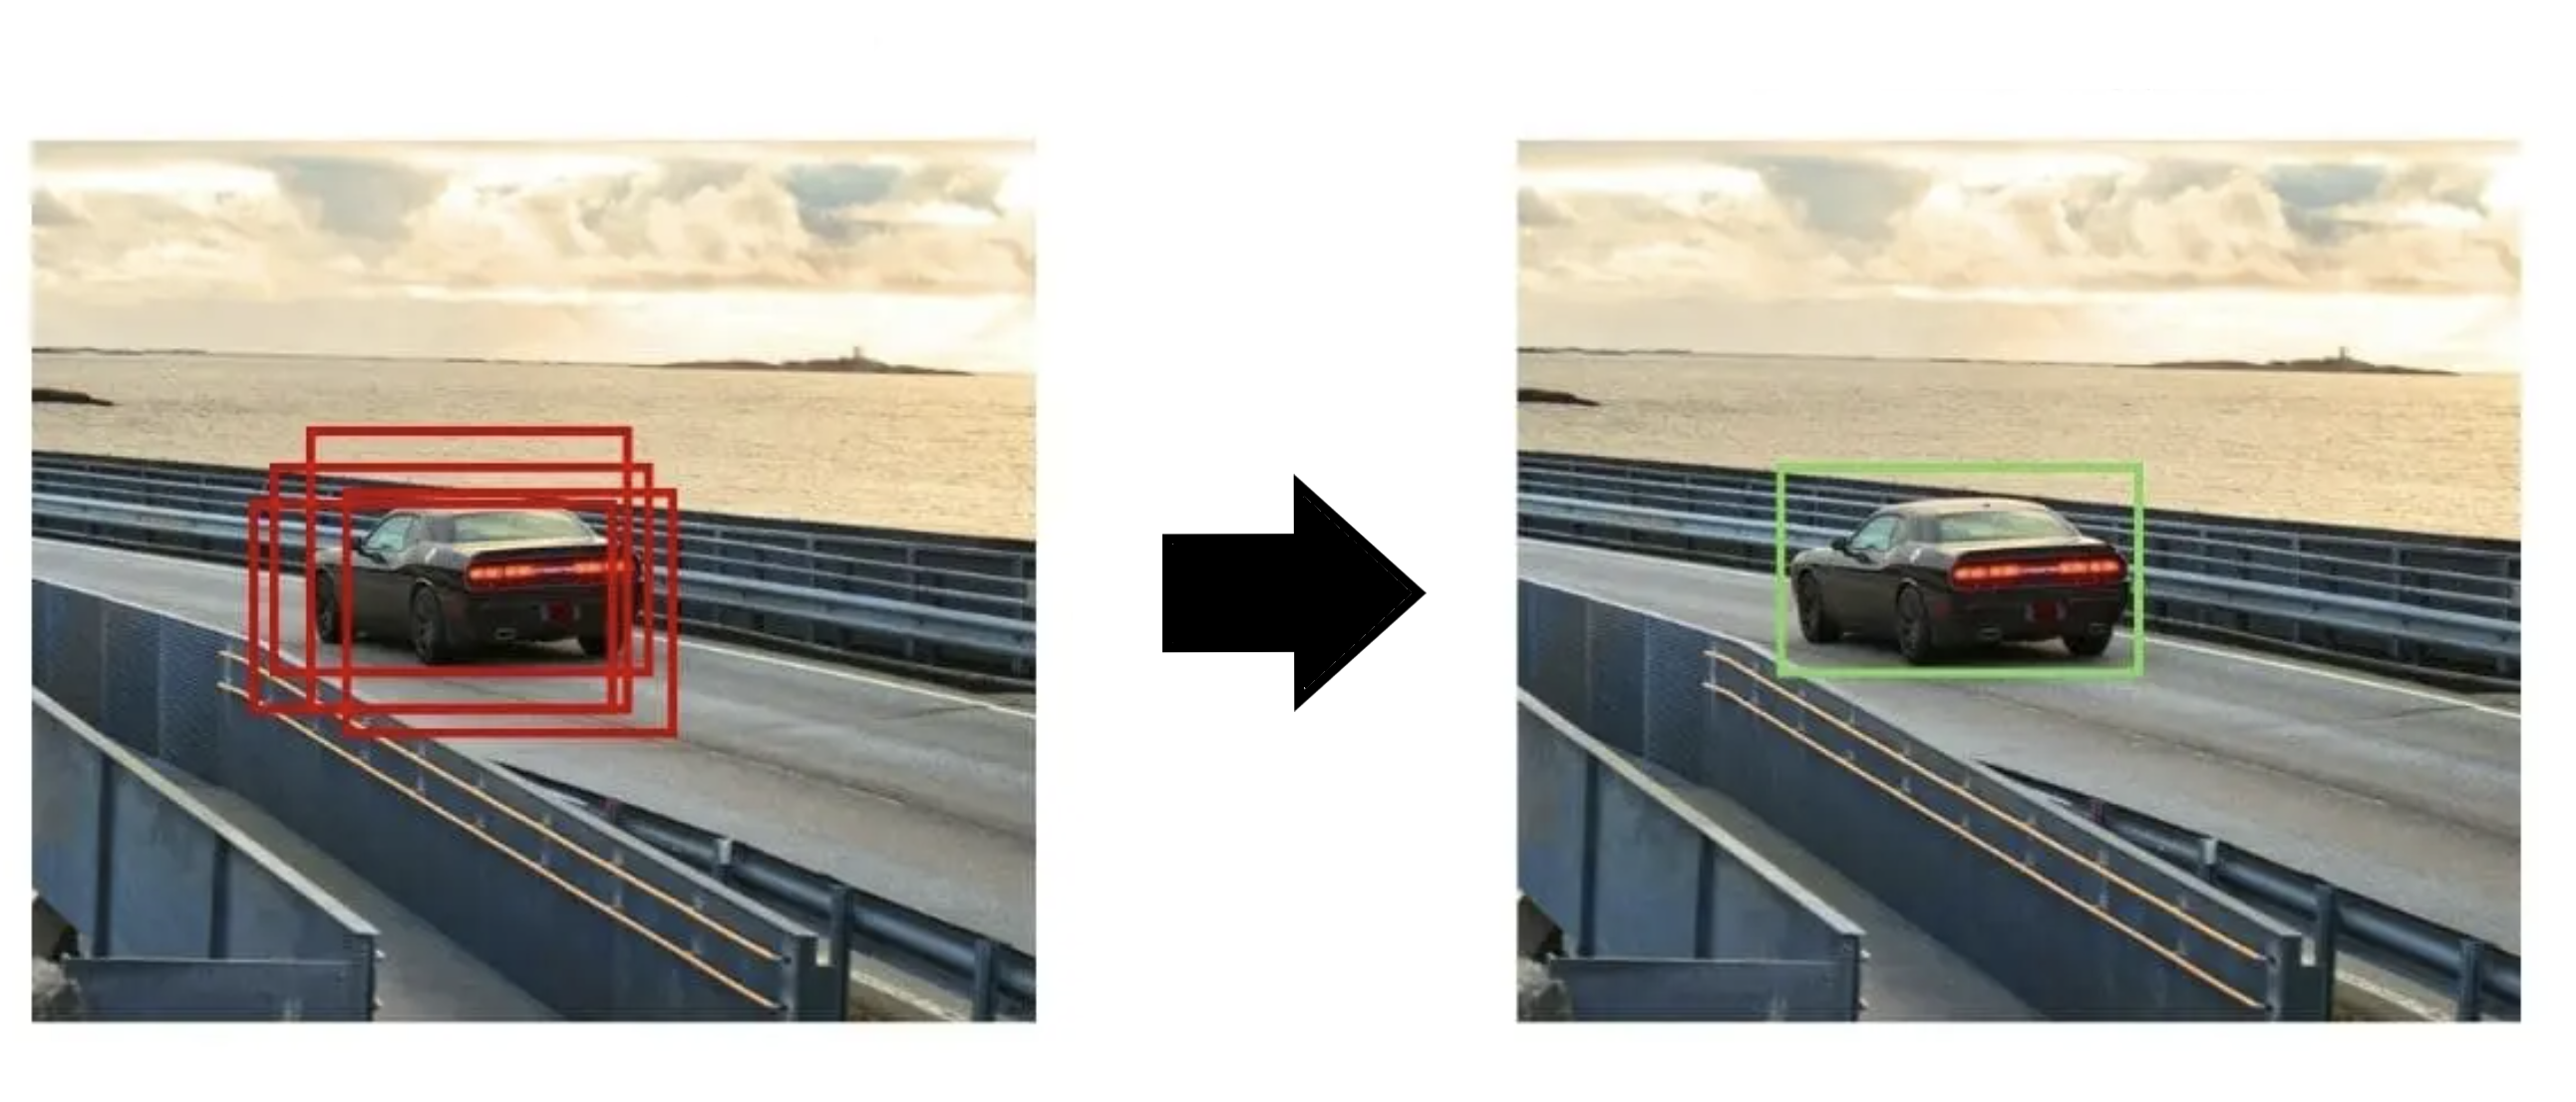
\includegraphics[width=0.8\linewidth]{figures/theory/image-recognition/nms.png}
    \caption[NMS before and after]{NMS before and after \cite{thepythoncode:nms}}
    \label{fig:nms}
\end{figure}






\subsection{Web}
\label{subsec:web}

\subsubsection*{Cross-Platform}
\label{subsubsec:corss-platform}

Cross-platform applications are software programs designed to function consistently across multiple operating systems or platforms. This includes desktop environments such as Windows, macOS, and Linux, as well as mobile platforms like iOS and Android. \cite{sevenpeaks:cross-platform}

\subsubsection*{Client-Server Architecture}
\label{subsubsec:client-server}

Client-server architecture is a network model in which multiple clients request and receive services from a centralized server over a local network or the Internet. Clients interact with the system through an application interface, while the server handles data processing. This architecture enables centralized control, scalability, and efficient resource management. See Figure~\ref{fig:client-server-architecture}. \cite{liquidweb:client-server}


\begin{figure}[h!]
    \centering
    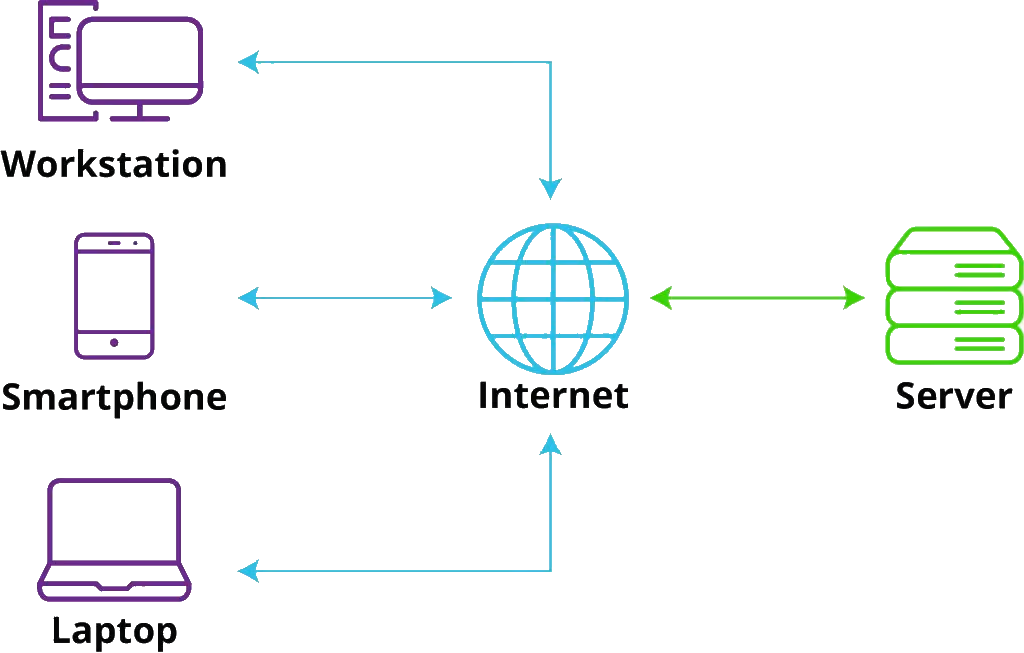
\includegraphics[width=0.75\linewidth]{figures/theory/client-server-architecture.png}
    \caption[Client-Server Architecture]{Client-Server Architecture \cite{liquidweb:client-server}}
    \label{fig:client-server-architecture}
\end{figure}

\subsubsection*{WebSocket}
\label{subsubsec:websocket}

WebSocket is a standardized communication protocol that enables full-duplex communication over a single \gls{tcp} connection, making it well-suited for real-time web applications. Unlike traditional \gls{http} requests — which follow a request-response model — WebSocket establishes a persistent connection that allows both the client and server to send and receive data at any time. This reduces the need for polling or long polling, significantly lowering network traffic and latency. As a result, WebSocket improves the efficiency and responsiveness of data transmission, particularly in applications such as live data feeds and online games. See Figure \ref{fig:websocket-vs-http} for a comparison. \cite{nodejs:websocket, apidog:websocket}


\begin{figure}[h!]
    \centering
    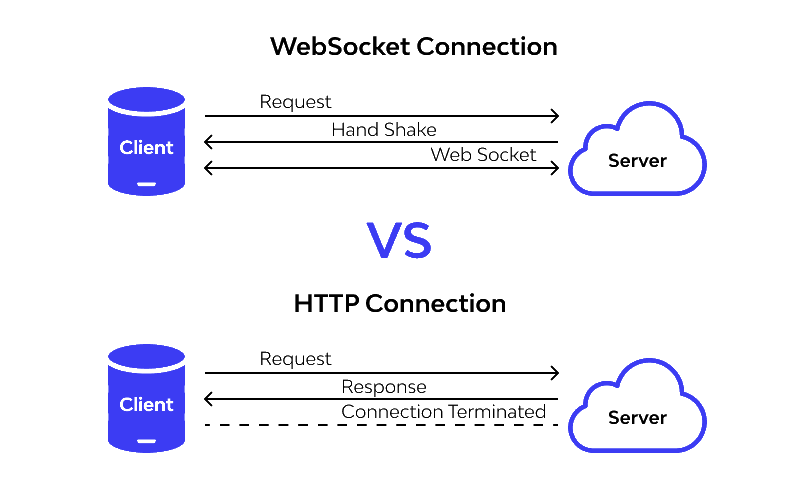
\includegraphics[width=0.75\linewidth]{figures/theory/websocket-vs-http.png}
    \caption[WebSocket Connection VS HTTP Connection]{WebSocket Connection VS HTTP Connection \cite{apidog:websocket}}
    \label{fig:websocket-vs-http}
\end{figure}

\section{Design}
\label{sec:design}

\subsection{Wireframe}
\label{subsec:wireframe}

A wireframe is a rough schematic created in the early stages of digital product design to help visualize and communicate the structure of a product or website. \cite{balsamiq:wireframe} \\

The same screen can be built in a lot of different ways, but only a few of them will get your message across correctly and result in an easy-to-use software or website. \cite{balsamiq:wireframe} \\

The purpose of a wireframe is to define a skeletal layout that is easy to understand, and encourages iteration and feedback. Getting to agreement on a good interface structure is a critical part of the software design process. \cite{balsamiq:wireframe} \\

Wireframes are important because doing this work now, before any code is written and before the visual design is finalized, will save you lots of time and painful vadjustment work later. \cite{balsamiq:wireframe} 

\subsection{WCAG}
\label{subsec:wcag}

\gls{wcag} provide technical specifications to improve the accessibility of websites and many other digital experiences. \cite{levelaccess:wcag}

\section{Code Quality}
\label{sec:code-quality}

\subsection{Code Review}
\label{subsec:code-review}

Code review is a critical step in the software development process, where a developer's implementation is examined by one or more peers before it is merged into an upstream branch, such as a feature branch or the main branch. This process provides a second opinion on the solution, helping to identify bugs, logic errors, uncovered edge cases, and other potential issues that may have been overlooked during development. \cite{gitlab:code-review} \\

A well-defined code review process is essential for maintaining high code quality and preventing unstable or faulty code from reaching production. By incorporating code reviews into the team's workflow, software development teams can foster continuous improvement, ensure that all code is reviewed by multiple perspectives, and reduce the risk of introducing defects into the codebase. \cite{gitlab:code-review} \\

Pull requests are a widely used mechanism to facilitate code reviews in modern version control systems. A pull request is a formal proposal to merge a set of changes from one branch into another. It provides a platform for collaborators to review, discuss, and approve changes before they are integrated into the main codebase. Pull requests also display the differences between the source and target branches, making it easier for reviewers to understand the proposed changes and provide constructive feedback. \cite{github:pr}

\subsection{Cohesion and Coupling}
\label{subsec:cohesion-and-coupling}

Cohesion and coupling are two fundamental concepts in software design that significantly impact the quality and maintainability of a system. \\

\begin{quote}
\textit{"\textbf{Cohesion} refers to the degree to which elements within a module work together to fulfill a single, well-defined purpose. \textbf{High cohesion} means that elements are closely related and focused on a single purpose, while \textbf{low cohesion} means that elements are loosely related and serve multiple purposes."} \cite{geeksforgeeks:c&c} \\
\end{quote}

\begin{quote}
\textit{"\textbf{Coupling} refers to the degree of interdependence between software modules. \textbf{Tight coupling} means that modules are closely connected and changes in one module may affect other modules. \textbf{Loose coupling} means that modules are independent, and changes in one module have little impact on other modules."} \cite{geeksforgeeks:c&c} \\
\end{quote}

\begin{figure}[h!]
    \centering
    \subfloat{{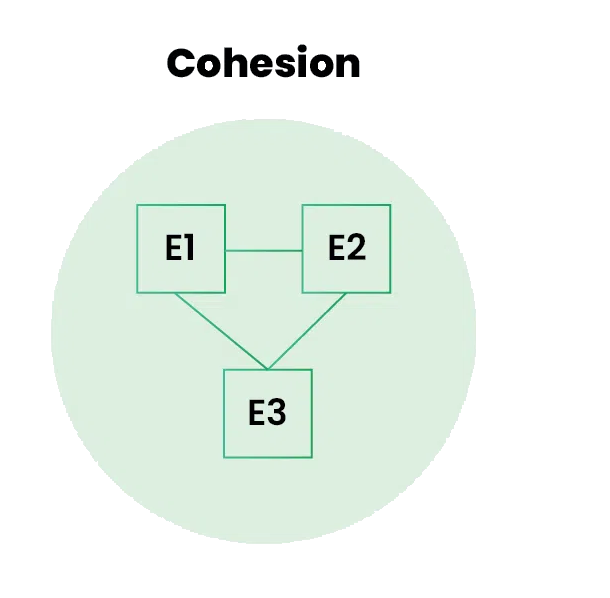
\includegraphics[width=0.5\linewidth]{figures/theory/cohesion.png}}}
    \subfloat{{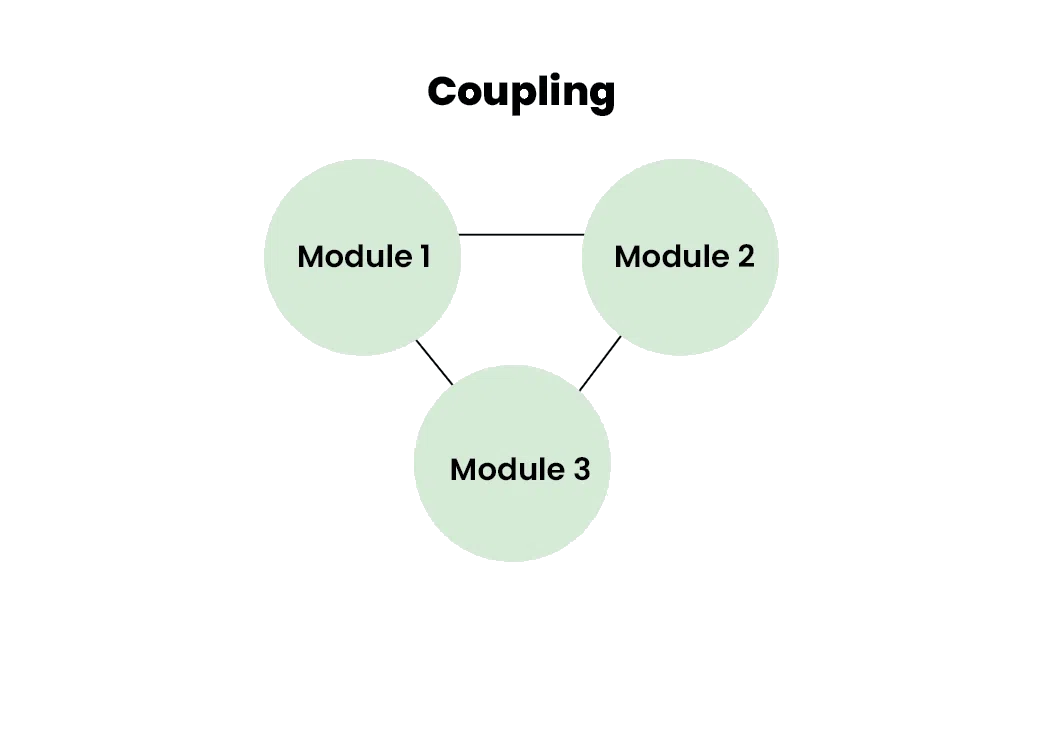
\includegraphics[width=0.5\linewidth]{figures/theory/coupling.png}}}

    \caption[Cohesion \& Coupling]{Cohesion \& Coupling \cite{geeksforgeeks:c&c}}
    \label{fig:cohesion-coupling}
\end{figure}

Both cohesion and coupling are important factors in determining the maintainability, scalability, and reliability of a software system. Tight coupling and low cohesion often result in systems that are difficult to change, test, and debug. Conversely, loose coupling and high cohesion contribute to systems that are modular, flexible, and easier to improve over time. An illustration of this concept is shown in Figure \ref{fig:cohesion-coupling}. \cite{geeksforgeeks:c&c}

\newpage

\subsection{Documentation}
\label{subsec:documentation}

Documentation is a critical component of software development, consisting of written materials that accompany a software program. It serves as a comprehensive reference for all stakeholders involved in the project, including developers, testers, and end-users. Documentation can take various forms, such as \gls{api} documentation, build instructions, user manuals, or internal design specifications. Its purpose is to provide clarity, facilitate understanding, and ensure the effective use and maintenance of the software. \cite{geeksforgeeks:doc} \\

High-quality documentation is essential for the success of any software project. It simplifies onboarding for new team members, aids in troubleshooting and debugging, and ensures that the software can be maintained and extended over time. Moreover, well-documented code and systems reduce the risk of knowledge loss when team members change or when revisiting older parts of the codebase. \cite{geeksforgeeks:doc} \\

In modern software development, documentation is not merely an afterthought but an integral part of the development process. It should be created and maintained alongside the code, ensuring that it remains accurate, up-to-date, and accessible to all relevant parties.

\subsection{Testing}
\label{subsec:testing}

\subsubsection*{Virtual Machine}
\label{subsubsec:virtual-machine}

Virtualization refers to the creation of a software-based — or "virtual" — version of a computer, with dedicated allocations of \gls{cpu}, memory, and storage drawn from a physical host machine or a remote server, such as one in a cloud provider's data center. A \gls{vm} is essentially a computer file that behaves like an independent computer system. It operates within a window as a separate computing environment, isolated from the host operating system. This isolation ensures that the software running inside the \gls{vm} cannot interfere with the host machine’s primary system. \cite{microsoft:virtual-machine}

\subsubsection*{Unit Testing}
\label{subsubsec:unit-testing}

Unit testing is a fundamental software testing technique in which individual units or components of a software application are tested in isolation. A unit typically refers to the smallest testable part of a program, such as a function, method, or class. The goal of unit testing is to validate that each unit performs as expected under various conditions, ensuring its correctness and reliability. \cite{geeksforgeeks:unit-test} \\

By identifying and addressing bugs early in the development cycle, unit testing significantly enhances code quality and reduces the cost of fixing issues later in the process. It is a core practice in \gls{tdd}, where tests are written before the actual code, promoting a disciplined approach to development and ensuring that the code meets its requirements from the outset. \cite{geeksforgeeks:unit-test} \\

Unit testing also contributes to the maintainability and scalability of a software system. Well-tested units are easier to refactor, extend, and integrate into larger systems, as their behavior is clearly defined and verified. Additionally, unit tests serve as living documentation, providing insights into how individual components are intended to function.

\subsubsection*{Usability Testing}
\label{subsubsec:usability-testing}

Usability testing is a critical aspect of software testing that focuses on evaluating a system from the perspective of an end user. Its primary goal is to determine how easily and effectively users can interact with the system to achieve their objectives. This type of testing involves observing representative users as they navigate through the product, identifying areas of confusion, difficulty, or inefficiency in the user experience. \cite{geeksforgeeks:user-test} \\

During usability testing, both qualitative and quantitative data are collected to assess the product's functionality and user satisfaction. Qualitative data, such as user feedback and observations, provides insights into user behavior and preferences. Quantitative data, such as task completion rates and time-on-task, offers measurable metrics to evaluate performance. Based on the findings, a detailed report is generated, outlining necessary improvements to enhance the product's usability. \cite{geeksforgeeks:user-test} \\

The ultimate goal of usability testing is to identify pain points in the user experience and uncover opportunities for improvement. By understanding how users interact with the product and where they encounter challenges, developers can make informed decisions to refine the design, improve functionality, and increase overall user satisfaction. \cite{geeksforgeeks:user-test}

\subsection{Type Safety}
\label{subsec:type-safety}

Type safety is a fundamental concept in software development that ensures the correctness of a codebase by detecting type-related errors during the development process. In dynamically typed languages, such as JavaScript, variables can be assigned values of any type, which often leads to subtle and hard-to-detect bugs. These bugs can be time-consuming to diagnose and resolve, particularly in large or complex codebases. Type safety addresses this issue by enforcing strict type constraints, thereby reducing the likelihood of runtime errors and improving overall code reliability. \cite{dev:type-safety}

\subsubsection*{Key Pillars of Type Safety}
\label{subsubsec:type-safety-pillars}

\begin{itemize}
    \item \textbf{Reliability:} Type safety acts as a protective mechanism, preventing runtime errors caused by type mismatches. By ensuring that variables and functions adhere to predefined types, it enhances the stability and reliability of applications. \cite{dev:type-safety}

    \item \textbf{Collaboration:} Explicit type declarations improve code readability and make it easier for developers to understand and work with each other's code. This fosters seamless collaboration, especially in team environments where multiple developers contribute to the same codebase. \cite{dev:type-safety}

    \item \textbf{Efficient Debugging:} Type safety enables early detection of type-related discrepancies, reducing the time and effort required for debugging. By catching errors at compile time (or during development in statically typed languages), it minimizes the risk of runtime failures and simplifies the debugging process. \cite{dev:type-safety}
\end{itemize}

In summary, type safety is a critical aspect of code quality, offering significant benefits in terms of reliability, collaboration, and debugging efficiency. Its implementation, whether through statically typed languages or tools like TypeScript, plays a vital role in modern software development practices. \cite{dev:type-safety}
